\documentclass{beamer}
\usetheme{Madrid}
\usecolortheme{dolphin}

\usepackage{amsmath,amssymb}
\usepackage{tikz}
\usepackage{pgfplots}
\usepackage{hyperref}

\title{Sample Beamer Presentation}
\subtitle{Converted to HTML with GitHub Actions}
\author{GitHub Actions Demo}
\institute{LaTeX to HTML Converter}
\date{\today}

\begin{document}

\begin{frame}
  \titlepage
\end{frame}

\begin{frame}{Outline}
  \tableofcontents
\end{frame}

\section{Introduction}

\begin{frame}{Introduction}
  \begin{itemize}
    \item This is a sample Beamer presentation
    \item It will be automatically converted to HTML
    \item The conversion preserves:
      \begin{itemize}
        \item Slide structure and navigation
        \item Mathematical equations
        \item TikZ diagrams
        \item Beamer themes and styles (to some extent)
      \end{itemize}
  \end{itemize}
\end{frame}

\section{Mathematical Equations}

\begin{frame}{Mathematical Equations}
  \begin{block}{Inline Math}
    The quadratic formula is $x = \frac{-b \pm \sqrt{b^2 - 4ac}}{2a}$ for a quadratic equation $ax^2 + bx + c = 0$.
  \end{block}
  
  \begin{block}{Display Math}
    The famous Euler's identity:
    \begin{equation}
      e^{i\pi} + 1 = 0
    \end{equation}
  \end{block}
\end{frame}

\begin{frame}{More Complex Equations}
  A more complex equation:
  \begin{align}
    \int_{-\infty}^{\infty} e^{-x^2} \, dx &= \sqrt{\pi} \\
    \sum_{n=0}^{\infty} \frac{1}{n!} &= e \\
    \prod_{i=1}^{n} i &= n!
  \end{align}
  
  A matrix example:
  \begin{equation}
    A = \begin{pmatrix}
      a_{11} & a_{12} & \cdots & a_{1n} \\
      a_{21} & a_{22} & \cdots & a_{2n} \\
      \vdots & \vdots & \ddots & \vdots \\
      a_{m1} & a_{m2} & \cdots & a_{mn}
    \end{pmatrix}
  \end{equation}
\end{frame}

\section{TikZ Diagrams}

\begin{frame}{Simple TikZ Shapes}
  \begin{figure}
    \centering
    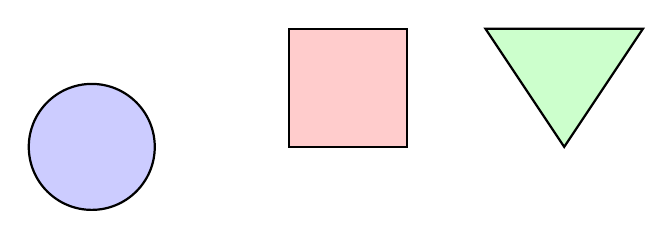
\begin{tikzpicture}
      \draw[thick, fill=blue!20] (0,0) circle (0.8cm);
      \draw[thick, fill=red!20] (2.5,0) rectangle (4,1.5);
      \draw[thick, fill=green!20] (6,0) -- (7,1.5) -- (5,1.5) -- cycle;
    \end{tikzpicture}
    \caption{Basic shapes in TikZ: circle, rectangle, and triangle}
  \end{figure}
\end{frame}

\begin{frame}{Function Plot}
  \begin{figure}
    \centering
    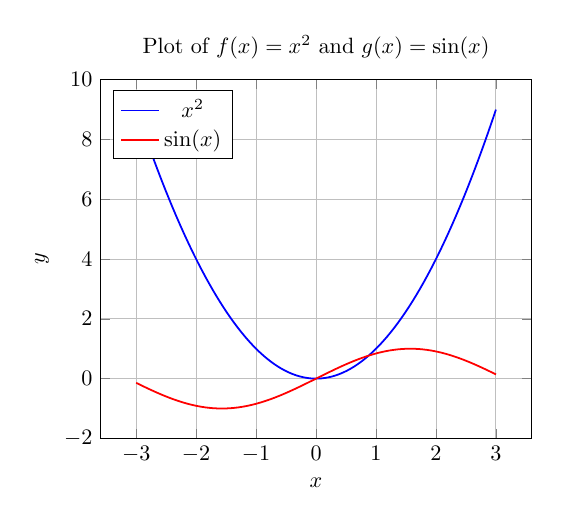
\begin{tikzpicture}[scale=0.8]
      \begin{axis}[
        xlabel={$x$},
        ylabel={$y$},
        title={Plot of $f(x) = x^2$ and $g(x) = \sin(x)$},
        legend pos=north west,
        grid=both,
        domain=-3:3,
        samples=100
      ]
        \addplot[blue, thick] {x^2};
        \addplot[red, thick] {sin(deg(x))};
        \legend{$x^2$, $\sin(x)$}
      \end{axis}
    \end{tikzpicture}
    \caption{Function plots using PGFPlots}
  \end{figure}
\end{frame}

\begin{frame}{Flowchart}
  \begin{figure}
    \centering
    \begin{tikzpicture}[node distance=1.5cm, auto, scale=0.7, transform shape]
      % Define styles
      \tikzstyle{decision} = [diamond, draw, fill=blue!20, text width=4.5em, text badly centered, inner sep=0pt]
      \tikzstyle{block} = [rectangle, draw, fill=blue!20, text width=5em, text centered, rounded corners, minimum height=4em]
      \tikzstyle{line} = [draw, -latex']
      
      % Place nodes
      \node [block] (init) {Initialize};
      \node [block, below of=init] (process) {Process};
      \node [decision, below of=process] (decide) {Decision?};
      \node [block, below left of=decide, xshift=-1.5cm] (yes) {Yes};
      \node [block, below right of=decide, xshift=1.5cm] (no) {No};
      \node [block, below of=yes, xshift=1.5cm] (end) {End};
      
      % Connect nodes
      \path [line] (init) -- (process);
      \path [line] (process) -- (decide);
      \path [line] (decide) -- node [near start] {yes} (yes);
      \path [line] (decide) -- node [near start] {no} (no);
      \path [line] (yes) |- (end);
      \path [line] (no) |- (end);
    \end{tikzpicture}
    \caption{A simple flowchart using TikZ}
  \end{figure}
\end{frame}

\section{Overlay Specifications}

\begin{frame}{Incremental Reveals}
  \begin{itemize}
    \item<1-> This is visible from step 1
    \item<2-> This is visible from step 2
    \item<3-> This is visible from step 3
    \item<4-> This is visible from step 4
  \end{itemize}
  
  \onslide<5->
  \begin{block}{Note}
    Overlay specifications are partially supported in the HTML conversion.
  \end{block}
\end{frame}

\begin{frame}{Highlighting}
  \begin{itemize}
    \item<1-| alert@1> This is highlighted on step 1
    \item<2-| alert@2> This is highlighted on step 2
    \item<3-| alert@3> This is highlighted on step 3
  \end{itemize}
  
  \begin{equation}
    e^{i\pi} + 1 = 0
  \end{equation}
\end{frame}

\section{Conclusion}

\begin{frame}{Conclusion}
  \begin{itemize}
    \item Beamer presentations can be automatically converted to HTML
    \item The conversion preserves most of the presentation features
    \item Mathematical equations are rendered with MathJax
    \item TikZ diagrams are converted to SVG
    \item The resulting HTML is responsive and works on different devices
  \end{itemize}
  
  \begin{block}{GitHub Actions Workflow}
    The GitHub Actions workflow handles the conversion process, organizes the output files, and deploys everything to GitHub Pages.
  \end{block}
\end{frame}

\begin{frame}{Thank You}
  \centering
  \Huge Thank You!
  
  \vspace{1cm}
  
  \large
  Check out the GitHub repository for more information.
\end{frame}

\end{document}